\documentclass[12pt, titlepage]{article}

\usepackage{booktabs}
\usepackage{tabularx}
\usepackage{hyperref}
\usepackage{pdflscape}
\usepackage{graphicx}
\usepackage{amsmath}
\usepackage{float}
\hypersetup{
    colorlinks,
    citecolor=blue,
    filecolor=black,
    linkcolor=red,
    urlcolor=blue
}
\usepackage[round]{natbib}

%% Comments

\usepackage{color}

\newif\ifcomments\commentstrue %displays comments
%\newif\ifcomments\commentsfalse %so that comments do not display

\ifcomments
\newcommand{\authornote}[3]{\textcolor{#1}{[#3 ---#2]}}
\newcommand{\todo}[1]{\textcolor{red}{[TODO: #1]}}
\else
\newcommand{\authornote}[3]{}
\newcommand{\todo}[1]{}
\fi

\newcommand{\wss}[1]{\authornote{blue}{SS}{#1}} 
\newcommand{\plt}[1]{\authornote{magenta}{TPLT}{#1}} %For explanation of the template
\newcommand{\an}[1]{\authornote{cyan}{Author}{#1}}

%% Common Parts

\newcommand{\progname}{ProgName} % PUT YOUR PROGRAM NAME HERE
\newcommand{\authname}{Team \#, Team Name
\\ Student 1 name
\\ Student 2 name
\\ Student 3 name
\\ Student 4 name} % AUTHOR NAMES                  

\usepackage{hyperref}
    \hypersetup{colorlinks=true, linkcolor=blue, citecolor=blue, filecolor=blue,
                urlcolor=blue, unicode=false}
    \urlstyle{same}
                                


\begin{document}

\title{System Verification and Validation Plan for \progname{}} 
\author{\authname}
\date{\today}
	
\maketitle

\pagenumbering{roman}

\section*{Revision History}

\begin{tabularx}{\textwidth}{p{3cm}p{2cm}X}
\toprule {\bf Date} & {\bf Version} & {\bf Notes}\\
\midrule
2025-02-27 & 1.0 & Initial Release\\
\bottomrule
\end{tabularx}

\newpage

\tableofcontents
\listoftables

\listoffigures

\newpage
\section{Symbols, Abbreviations, and Acronyms}

\renewcommand{\arraystretch}{1.2}
\begin{tabular}{l l} 
  \toprule		
  \textbf{symbol} & \textbf{description}\\
  \midrule
  a & arbitrary positive integer\\
  CAS & Computing and Software\\
  CI & Continuous Integration\\
  CSV & Comma-Separated Values\\
  DE & Domain Expert \\
  $d_{total}$ & bin size, or number of binary descriptions \\
  $D_{bin}$ & 1D array of 32 byte binary strings \\
  FOV & field-of-view\\
  $I$ & 2D array of pixel values for a greyscale image \\
  $I'$ & transformed 2D array of pixel values\\
  $IFC$ & Image Feature Correspondences\\
  $k$ & number of total keypoints\\
  LD & Lead Developer \\
  $m$ & horizontal image dimension\\
  MG & Module Guide \\
  MIS & Module Interface Specification\\
  $n$ & vertical image dimension\\
  ORB & Oriented FAST and Rotated BRIEF\\
  $p$ & patch size\\
  PEP8 & Python Enhancement Proposal-8\\
  PNG & Portable Network Graphic\\
  PS & Project Supervisor\\
  RGB & Red-Green-Blue coloured imagery\\
  SDI & Software Design Instructor\\
  SLAM & Simultaneous Localization and Mapping\\
  SRS & Software Requirements Specification\\
  $t$ & intensity threshold \\
  VnV & Verification and Validation\\
  $\sigma$ & standard deviation\\
  \bottomrule
\end{tabular}\\

\newpage

\pagenumbering{arabic}
\noindent The intent of this document is to define the Verification and Validation (VnV) processes
that will be used to assess \progname, (IFC) software. Specifically, this document will be used to 
characterize the behaviour and performance of this software. The remaining sections of this document 
outline a detailed summary of the specific objectives of the VnV campaign. This includes considerations 
for the scope of the VnV efforts with respect to contraints that stem from the Winter 2025
development schedule, as well as anticipated activities for the Summer 2025 development cycle.
Verification procedures are present for select deliverables and milestone, and include 
an overview of anticipated cases for both system tests unit tests.

\section{General Information}

\subsection{Summary}
The Image Feature Correspondences (IFC) software is a feature comparison algorithm that is intended 
to be used as part of a pipeline to perform extrinsic camera calibration for 
applications in mobile robotics. It accepts camera configuration parameters and greyscale imagery data at 
different poses to identify common features amongst collected images. 

\subsection{Objectives}
The VnV process is intended to characterize how well the for the IFC software performs in its 
intended capacity to identify features amongst collected imagery. The performance of this system 
can vary significantly as it is influenced by factors such as overlap in camera fields-of-view (FOV),
the observed contrast between objects in an image, and variance in scale, rotation, and ambient 
illumination conditions. Furthermore, as there is no common baseline to compare this software to as 
an oracle, the VnV campaign for the IFC software is intended to characterize the performance of the 
integrated image processing functions against a set of test datasets. Key objectives of this process 
are defined below.

\begin{itemize}
  \item assess the reliability in the feature matching pipeline
  \item assess how users perceive their interactions with the IFC software 
  \item characterize the performances of the IFC software with metrics such as processing time and 
  memory usage
  \item cross-validate the performance of the IFC software with accepted benchmarked datasets
\end{itemize}
Verification of the individual functions within the OpenCV library themselves falls outside of the 
scope of this project, as we can assume that the library has been verified by its own 
implementation team. 
\\ \\

\subsection{Challenge Level and Extras}
% Updated to clearly indicate the challenge level of the project and how it consitutes the first portion of a larger image processing pipeline for MASc studies.
The proposed software constitutes a research project, as the IFC software serves as the front end of a robust optimization framework 
for extrinsic camera calibration. The IFC software must be capable of handling large volumes of high-resolution imagery while ensuring reliability through consistent and repeatable outputs. The software will be designed for robustness in data processing, accommodating a wide range of input conditions. Additionally, it will maintain a streamlined user experience, allowing users to override select default parameters while ensuring that the learning curve remains minimal for efficient adoption. 

As the long-term goal for this software is to absorb it into a larger calibration pipeline for research in the domain of mobile robotic, this project is defined as an advanced level of challenge. This program will supply a set of installation instructions, source code, test scripts, test imagery, and verification report. No additional documentation, such as a user manual will be provided.

\subsection{Relevant Documentation}
Relevant documentation has been hyperlinked throughout the length of the document. This enables 
the reader to access each resource within the context of the section that the reference is invoked.
\begin{itemize}
\item \textbf{Software Requirements Specification \href{https://github.com/KiranSingh15/CAS-741-Image-Correspondences/blob/main/docs/SRS/SRS.pdf}
{(SRS)}}
\item \textbf{Module Guide \href{https://github.com/KiranSingh15/CAS-741-Image-Correspondences/blob/main/docs/Design/SoftArchitecture/MG.pdf}
{(MG)}} 
\item 
\textbf{Module Interface Specification \href{https://github.com/KiranSingh15/CAS-741-Image-Correspondences/blob/main/docs/Design/SoftDetailedDes/MIS.pdf}{(MIS)}}
\end{itemize}

Additional document includes the checklists as follows.
\begin{itemize}
\item \textbf{\href{https://github.com/KiranSingh15/CAS-741-Image-Correspondences/blob/
main/docs/Checklists/SRS-Checklist.pdf}
{SRS Checklist}}. 
\item \textbf{\href{https://github.com/KiranSingh15/CAS-741-Image-Correspondences/blob/main/docs/Checklists/MG-Checklist.pdf}
{MG Checklist}} 
\item \textbf{\href{https://github.com/KiranSingh15/CAS-741-Image-Correspondences/blob/main/docs/Checklists/MIS-Checklist.pdf}{MIS Checklist}}
\item \textbf{\href{https://github.com/KiranSingh15/CAS-741-Image-Correspondences/blob/main/docs/Checklists/VnV-Checklist.pdf}
{VnV Checklist}}
\end{itemize}

\section{Plan}
This section outlines how each aspect of the VnV effort will be performed. This may be handled by 
milestone or by general practices, such as continuous integration and linters. 

\subsection{Verification and Validation Team}
The VnV team consists of four members, each of whom play a distinct role in the 
verification process. These roles and responsibilities are outlined in Table \ref{Table_Ver_Roles}.

\begin{table}[tbp!]
  \centering
  \begin{tabular}{|p{0.11\linewidth}|p{0.24\linewidth}|p{0.6\linewidth}|} 
    \hline
    \textbf{Name} & \textbf{Role} & \textbf{Description}\\
    \hline
    Kiran Singh & Lead Developer and Test Designer (LD) & Responsibilities include the
    identification of critical business cases for integrated tests, assessment of 
    schedule and scope considerations,  design and implementation of unit tests, 
    system tests, and documentation of test results.\\
    \hline
    Matthew Giamou & Project Supervisor (PS) & Lead consultant on integrated 
    performance needs and decomposition for software modules. Responsibilities 
    include review of proposed VnV scope, as proposed by 
    Kiran S., and provision of feedback to the general scope of the VnV campaign, and approval 
    of the individual test cases that are proposed by the LD. \\
    \hline
    Aliyah Jimoh & Domain Expert (DE) & Responsibilities include provision of 
    feedback on proposed test cases for the 
    scope of test cases for both the functional and non-functional requirements. They 
    will also provide feedback on the code walkthrough per the final CAS 741 presentation. 
    This statisfies the need for a reviewer that is removed from the design effort yet
    still holds sufficient domain knowledge to provide feedback on the overall design 
    and associated VnV efforts.\\ 
    \hline
    Spencer Smith & Software Development Instructor (SDI) & Responsibilities include 
    provision of feedback on proposed test cases for the scope of test cases 
    for both the functional and non-functional requirements. They will also 
    provide feedback on the code walkthrough per the final CAS 741 presentation. 
    This reviewer provides an essential stream of feedback as they are fully removed 
    from the application domain and may willing to question assumptions and address biases 
    that may be implicit amongst other members of the VnV team.\\
    \bottomrule
  \end{tabular}\\
  \caption{Roles and Responsibilities of the Verification and Validation Team}
  \label{Table_Ver_Roles}
\end{table}


\subsection{SRS Verification Plan}
The \textbf{\href{https://github.com/KiranSingh15/CAS-741-Image-Correspondences/blob/main/docs/SRS/SRS.pdf}
{SRS}} shall be reviewed by each member of the reviewer team to form consensus that the SRS has been correctly 
decomposed into sufficient requirements.
\begin{itemize}
\item the models are deemed to be comprehensible
\item the models are deemed to be correct
\item the associated requirements are traced correctly with respect to the models 
and project scope 
\item the requirements are decomposed in a manner that facilitates verification
\end{itemize}
Feedback on the \textbf{\href{https://github.com/KiranSingh15/CAS-741-Image-Correspondences/blob/main/docs/SRS/SRS.pdf}
{SRS}}
 from the DE and SDI will be captured through 
the use of Github Issues. Specifically, both reviewers will use the 
\textbf{\href{https://github.com/KiranSingh15/CAS-741-Image-Correspondences/blob/
main/docs/Checklists/SRS-Checklist.pdf}
{SRS Checklist}}. 
The lead developer will respond in turn to each issue and if 
reserves the right to reject a proposed change as needed. \\
The Lead Developer will schedule a meeting with the Project Supervisor to walk through 
the first revision of the \textbf{\href{https://github.com/KiranSingh15/CAS-741-Image-Correspondences/blob/main/docs/SRS/SRS.pdf}
{SRS}}
 document. In this meeting, the Project Supervisor will offer 
feedback and recommendations for candidate revisions to the outlined models and requirements. 
The Lead Developer will then create issues in Github to address each proposed revision.

\subsection{Design Verification Plan}
The DE and SDI will review the Module Guide 
\textbf{\href{https://github.com/KiranSingh15/CAS-741-Image-Correspondences/blob/main/docs/Design/SoftArchitecture/MG.pdf}
{(MG)}} and the Module Interface Specification 
\textbf{\href{https://github.com/KiranSingh15/CAS-741-Image-Correspondences/blob/main/docs/Design/SoftDetailedDes/MIS.pdf}
{(MIS)}} against the 
\textbf{\href{https://github.com/KiranSingh15/CAS-741-Image-Correspondences/blob/main/docs/Checklists/MG-Checklist.pdf}
{MG Checklist}} and
\textbf{\href{https://github.com/KiranSingh15/CAS-741-Image-Correspondences/blob/main/docs/Checklists/MIS-Checklist.pdf}
{ Checklist}}. The objective of this review cycle is to ensure that the design of the system:
\begin{enumerate}
\item is unambiguous
\item adheres to best-practices of module design
\item aligns with the requirements as identified in the 
\textbf{\href{https://github.com/KiranSingh15/CAS-741-Image-Correspondences/blob/main/docs/SRS/SRS.pdf}
{SRS}}
\end{enumerate}


\subsection{Verification and Validation Plan Verification Plan}
The VnV Plan will be verified via inspection by the DE and the 
Software Development Instructor. The 
\textbf{\href{https://github.com/KiranSingh15/CAS-741-Image-Correspondences/blob/main/docs/Checklists/VnV-Checklist.pdf}
{VnV Plan Checklist}} 
will be used as the assessment criteria for the inspection. 
Feedback will provided as Github issues and will be handled in the same manner as feedback 
for the SRS.\\ \\

% Removed discussion of mutation testing due to schedule constraints.

\subsection{Implementation Verification Plan}
The IFC software shall be verified against the test procedures outlined in Sections \ref{FR_Tests} and 
\ref{NFR_Tests}. Static verification of the IFC software will consist of a code walkthrough. This will take 
place during the CAS 741 final presentation, where the DE and SDI will have the opportunity to observe 
the code and raise issues following the presentation via GitHub. \\ \\
Dynamic verification of the IFC software will consist of system and unit tests via PyTest. System tests 
are outlined in Section \ref{Sys_Tests}. Unit tests will be outlined in Rev 2 of the VnV Plan in 
Section \ref{UTD}.

\subsection{Automated Testing and Verification Tools}
Several tools will be used to support automated testing and verification. They include:
\begin{itemize}
\item Continuous Integration (CI) will be facilitated via GitHub Actions. A pull request will be used 
to run automated tests.
\item Pytest will be used to execute system tests, unit tests, and to assess code coverage. 
\item flake8 will be used as a linter to ensure adherence to PEP8 standards. 
% Pylint has been removed in favour of flake8
\end{itemize}

\subsection{Software Validation Plan}
% Updated per Instructor feedback on Rev 1.0
Validation testing has been identified as out of scope for the IFCS software.

\section{System Tests}\label{Sys_Tests}
This section outlines the general roadmap for the required integrated system tests. 
\subsection{Tests for Functional Requirements} \label{FR_Tests}
This section outlines the system tests that verify the requirements outlined in 
Section 5 of the 
\textbf{\href{https://github.com/KiranSingh15/CAS-741-Image-Correspondences/blob/main/docs/SRS/SRS.pdf}
{SRS}}. 

\begin{figure}[h!]
  \begin{center}
   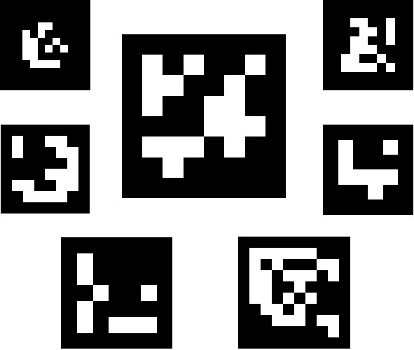
\includegraphics[width=0.6\textwidth]{images/ArUco_Field_Gen.jpg}
  \caption[An example of a generated ArUco pattern]{An example of a generated ArUco pattern. Image taken 
  from \cite{ARUCO_Markers_openCV}}
  \label{gen_aruco} 
  \end{center}
\end{figure}

\begin{figure}[h!]
  \begin{center}
   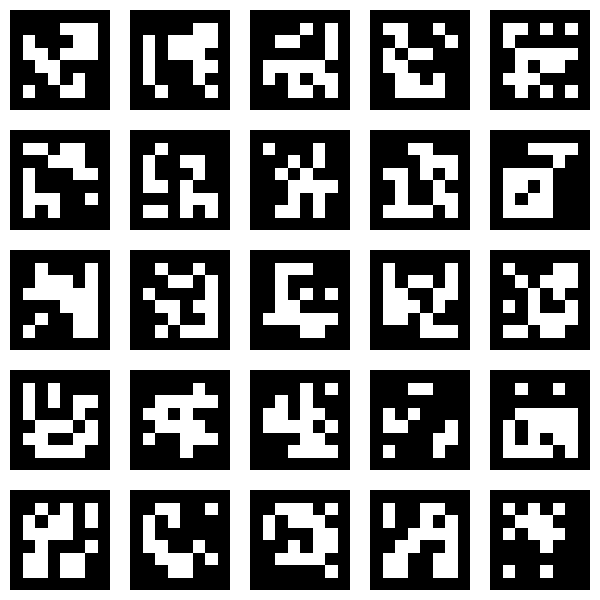
\includegraphics[width=0.6\textwidth]{images/aruco_000.png}
  \caption[An example of ArUco patterns within the scene of a captured greyscale image]
  {Expected baseline ArUco pattern for functional tests STFR-IS-01, STFR-KP-01, STFR-FD-01, and STFR-FM-01}
  \label{gs_aruco_field} 
  \end{center}
\end{figure}

\subsubsection{Feature Detection}
This test section is intended to assess that the system can accept new parameters from users and covers 
requirements R1 through R7 and R9 through R11, in Section 5.1 of the 
\textbf{\href{https://github.com/KiranSingh15/CAS-741-Image-Correspondences/blob/main/docs/SRS/SRS.pdf}
{SRS}}. 
		
\paragraph{Image Smoother}
\begin{enumerate}
\item \hypertarget{STFR-IS-01}{\textbf{STFR-IS-01}}

\textbf{Requirements Addressed:} R1, R5, R9

\textbf{Control:} Automated		

\textbf{Initial State:} Uninitialized

\textbf{Input:} Generated binary patterned fiducial markers, named 
\href{https://docs.opencv.org/4.x/d5/dae/tutorial_aruco_detection.html}
{ArUco} markers, will be used as simplified targets for corner detection. The script that is used to generate these images is provided in the src code, \href{https://github.com/KiranSingh15/CAS-741-Image-Correspondences/blob/main/src/tests/gen_arcuo.py}{gen\_aruco.py}.A depiction of these markers is shown in Figure \ref{gen_aruco}. This script generates an initial image with contains 25 $6\times 6$-bit ArUco markers. It uses a seed of 42 to perform scaling, rotational, and translational transforms on the baseline marker. These transforms range between $-45^\circ$ and $45^\circ$, 30 pixels of lateral translation, and a scaling factor between 0.5 and 0.9. A total of 20 transformed images are produced as inputs for the test. Each image $I$ is defined as a 2D image of $600 \times 600$ pixel resolution. A Gaussian smoothing kernel of 5 and standard deviation of 1.0 will be used to smooth the edges of the imagery. 

\textbf{Output:} 20 output images as a 2D array, each of which have a descriptive name that clearly identifies the input image from which it originates. In this case, all images should use the convention of 'aruco\_xxx.png', where 'xxx' represents the enumerated ID of the ArUco marker. The output image, $I'$, should be of equal size and the same data type as its 
corresponding image $I$. All images should be saved under a distinct folder to prevent mixing of input and output imagery.

\textbf{How test will be performed:} Automated Tools (i.e. Pytest). If the ArUco imagery is not provided in the src/tests folder, then the user needs to run the gen\_aruco.py script to generate the test imagery. Once complete, the user needs to only run STFR-IM-01.py via Pytest while in the src folder to run the test. The pytest file then checks each generated image to confirm that it has the same size and image datatype as the original input image. If each image has a resolution of $600 \times 600$ pixels and is an image of type unit8, then the test is considered a pass.

\end{enumerate}


\paragraph{Keypoint Detector}
\begin{enumerate}
\item \hypertarget{STFR-KP-01}{\textbf{STFR-KP-01}\\}
\textbf{Requirements Addressed:} R2, R6, R10

\textbf{Control:} Automatic	

\textbf{Initial State:} Uninitialized			

\textbf{Input:} A collection of 20 smoothed PNG images $I'$ with a resolution of $600\times 600$ that 
contain the same ArUco markers as outlined in System Test \hyperlink{STFR-IS-01}{STFR-IS-01}. The user assigns a pixel intensity threshold ($t$) of 60.

\textbf{Output:} A flag which indicates that corner detection is active. 
A 2D array of size ${k \times m}$, where $k$ is the quantity of identified keypoints and the first and second columns are populated with the horizontal and vertical coordinates for each keypoint. Each entry in the array should be rounded to a positive integer value. Any outstanding columns may be populated with associated metadata as a product of the selected method of keypoint detection. For example, oriented FAST (o-FAST) differs from standard FAST in that it also provides an measure of rotation for each keypoint as an additional column. Each array should have a unique title that clearly defines the original image from which its keypoints were identified. All output arrays should be saved to a unique folder to separate them from the input images.

\textbf{How test will be performed:} Automated Tools (i.e. Pytest)If the smoothed ArUco imagery is not provided in the src/tests folder, then the user needs to run the gen\_aruco.py script to generate the test imagery. Once complete, the user needs to only run STFR-KP-01.py via Pytest while in the src folder to run the test. The Pytest file then checks each row of the generated CSV file to confirm that each x and y coordinate is rounded to an integer value. If any keypoint does not contain either an x or y coordinate, a flag is raised and is reported. If all x and y coordinates are rounded to the nearest integer, then the test is deemed to be a pass.
\end{enumerate}

\paragraph{Feature Definition}
\begin{enumerate}
\item \hypertarget{STFR-FD-01}{\textbf{STFR-FD-01}\\}
\textbf{Requirements Addressed:} R3, R4, R7, R11

\textbf{Control:} Automatic

\textbf{Initial State:} Uninitialized

\textbf{Input:} A collection of 20 PNG images with a resolution of $600\times 600$, where each image features 25 $6\times 6$ ArUco markers within the scene. A $k\times m$ 2D array will be provided for each image, where $k$ is the number of keypoints within each image. A target bin size ($d_{total}$) of 100 will be used to define the target number of feature descriptors. A patch size ($p$) of 31 will be used to define the adjacent region of a keypoint for which to define descriptors.

\textbf{Output:} $D_{bin}$, an array of length $d_{total}$ with a minimum width of 1 where all entries of the array are 32 byte binary strings. The width of this array may be increased if associated horizontal and vertical coordinates for the corresponding keypoint may be affixed to each descriptor. 

\textbf{Test Case Derivation:} \href{https://sites.cc.gatech.edu/classes/AY2024/cs4475_summer/images/ORB_an_efficient_alternative_to_SIFT_or_SURF.pdf}
{ORB: An efficient alternative to SIFT or SURF}. This publication outlines methods to develop and the corresponding assessment of binary feature descriptors.

\textbf{How test will be performed:} Automated Tools (i.e. Pytest). If the smoothed ArUco imagery is not provided in the src/tests folder, then the user needs to run the gen\_aruco.py script to generate the test imagery. Once complete, the user needs to only run test\_STFR-FD-01.py via Pytest while in the src folder to run the test. The Pytest file then checks each row of the generated CSV file to confirm that each descriptor has a horizontal and vertical coordinate, rounded to the nearest integer. All 256 bits of the binary descriptor are then checked to ensure that there is no data bit loss from conversion to CSV. If associated horizontal or vertical coordinates are identified as missing, then the test fails. If there is any loss of databit within the 32 byte descriptor, then the test fails. If all identified descriptors pass both the coordinates and descriptor bitwise checks, then the test is defined to be a pass.
\end{enumerate}

\subsubsection{Feature Comparison}

This test section is intended to assess that the system can accept new parameters from users. It addresses 
requirements R8 and R12 through R15 in Section 5.1 of the 
\textbf{\href{https://github.com/KiranSingh15/CAS-741-Image-Correspondences/blob/main/docs/SRS/SRS.pdf}
{SRS}}. 
		
\paragraph{Descriptor Comparison}
\begin{enumerate}
\item \hypertarget{STFR-DC-01}{\textbf{STFR-DC-01}\\}
\textbf{Requirements Addressed:} R8, R12, R13, R14, R15

\textbf{Control:} Automated		

\textbf{Initial State:} Uninitialized

\textbf{Input:} 20 1D arrays, each which have a unique length, $D_{bin}$, where each element of the 
array is a 32 byte binary string known as a binary descriptor. Each array should be labeled with a 
descriptive name that clearly references the instance of both the camera and pose at the time of image 
capture.

\textbf{Output:} A flag that indicates that Hamming Distances were compared. A dynamically-sized array, stored as a Pandas dataframe, where the length of the array is the number of matched features. The columns of the array will include the properties as follows.
\begin{itemize}
\item Binary descriptors of both features as 32 byte binary strings
\item Corresponding image IDs for each feature
\item Matching scores between both features
\item The Hamming Distance of each candidate match between features
\end{itemize}
% Introduced to address the question of "What is the Correct Hamming Distance?" per feedback on Rev 1.0
Note that we do not compare the identified Hamming Distance as there is no baseline Hamming Distance for which to compare. \\

\textbf{How test will be performed:} Automated Tools (i.e. Pytest)
If the smoothed ArUco imagery is not provided in the src/tests folder, then the user needs to run the gen\_aruco.py script to generate the test imagery. Once complete, the user needs to only run test\_STFR-FM-01.py via Pytest while in the src folder to run the test. The Pytest file then checks each row of the generated CSV file to confirm that for both pairs of descriptors that compose a candidate match, each descriptor has a horizontal and vertical coordinate, rounded to the nearest integer. All 256 bits of the binary descriptor are then checked to ensure that there is no data bit loss from conversion to CSV. Finally, the calculated distance between each descriptor is assessed to confirm that it is a positive integer. If associated horizontal or vertical coordinates are identified as missing, then the test fails. If there is any loss of databit within the 32 byte descriptor, then the test fails. If the distance between descriptors is not a positive integer, the test fails. If all identified descriptors pass both the coordinates and descriptor bitwise checks, and the distance is a positive integer, then the test is defined to be a pass.
\end{enumerate}

\subsection{Tests for Nonfunctional Requirements}\label{NFR_Tests}
\subsubsection{Reliability}
The IFC software is envisioned to be used as part of the front end of a larger camera calibration pipeline, 
where the outputs of the IFC software need to produce consistent results for use in a back-end optimization 
module. Therefore, the IFC software needs to undergo verification to ensure that it can match the same 
features between two images. The following system test satisfies \textbf{NFR1} of the 
\textbf{\href{https://github.com/KiranSingh15/CAS-741-Image-Correspondences/blob/main/docs/SRS/SRS.pdf}
{SRS}}.

\paragraph{Repeatability}
\begin{enumerate}
\item \hypertarget{STNFR-RE-1}{\textbf{STNFR-RE-1}\\}
\textbf{Type: Dynamic}

\textbf{Initial State:} Uninitialized

\textbf{Input/Condition:} Two datasets of imagery data. These datasets contain the same collection of images, 
but are arranged in a different order.

\textbf{Output/Result:} The feature matching pipeline will be use to identify features and compare them amongst 
images for both datasets. For both datasets, a dynamically-sized array will be output. These arrays will 
contain the feature descriptors and the image IDs of origin, as specified in as specified in 
\hyperlink{STFR-DC-01}{STFR-DC-01}. 
One array will be reordered to reflect the order of the other array. Once the second array has been reordered, 
the arrays will be compared in terms of their length and contents. For example, in images A and B, they will be 
processed under the pseudonym of B' and A', respectively. That is, for each feature of A, its descriptor and x-y 
coordinates are equivalent to those of B'. Similarly, the coordinates and descriptor of B are equivalent to A'. 
The features of A and B will be compared to identify matches. Then the features of A' and B' will be compared as 
well. The test will be considered a pass if the identified matches between A and B share the same descriptors and 
coordinates as the identified matches between B' and A', respectively.

\textbf{How test will be performed:} PyTest. Two sample images from the Lego library have been duplicated and reordered with new names. Paths to the original and transformed images are outlined in the  test\_STFR-RE-01.py file. A script will assess that for the corresponding transformed image, that the same coordinates and 32-byte feature descriptor are identified as a match candidate with the same coordinates and 32-byte descriptor of the transformed image for the complementary image.
\end{enumerate}

\subsubsection{Usability}
As part of a larger pipeline, the IFC software needs to be simple for its users to integrate into the calibration system. 
This may be reflected in the perception of how simple it is for the user to 
implement its on their own system and to run the program as its own module. This usability criterion is 
reflected in \textbf{NFR2} of the 
\textbf{\href{https://github.com/KiranSingh15/CAS-741-Image-Correspondences/blob/main/docs/SRS/SRS.pdf}
{SRS}}.

\paragraph{User Experience: End-to-End Feature Matching}
\begin{enumerate}
\item \hypertarget{STNFR-UX-1}{\textbf{STNFR-UX-1}\\}
\textbf{Type:} Dynamic

\textbf{Initial State:} Uninitialized

\textbf{Output/Result:} A dataframe of identified features, as outlined in \hyperlink{STFR-DC-01}{STFR-DC-01}. 
Once the test has been completed, the user will be asked to express their opinion of their experience of the 
system, and to remark on the following topics.
\begin{itemize}
\item the degree of perceived difficulty in preparing the input files
\item the degree of perceived difficulty in assignment of the camera properties
\item the user's overall satisfaction with using the program
\end{itemize} 

\textbf{How test will be performed:} Dynamic Test by User
\end{enumerate}
The characteristics of the desired user are outlined in the \textbf{\href{https://github.com/KiranSingh15/CAS-741-Image-Correspondences/blob/main/docs/SRS/SRS.pdf}{SRS}}. However, for the intent of testing, the user may be defined as the Project Supervisor or Domain Expert. The user will be provided a collection of images from different cameras. Each image will be labelled with 
a descriptive title that clearly defines what camera the image originates from. The user shall be responsible 
to insert all images into a common folder.

The user shall execute the following procedure in the following order.
\begin{enumerate}
  \item The user shall open the directory to the IFC configuration file.
  \item In the IFC program configuration file, the user shall:
  \begin{enumerate}
      \item Update the input location as the folder of all the input images.
      \item Update the system directory with the desired location of the matched feature array.
      \item Assign a directory for altered imagery, if desired.
      \item Input the number of cameras per the sized camera data.
      \item Provide the following details for each camera:
      \begin{enumerate}
          \item A descriptive name of the camera that matches the prefix of the name of its imagery data.
          \item The resolution of each camera.
      \end{enumerate}
  \end{enumerate}
  \item The user shall close the IFC configuration file.
  \item The user initiates execution of the feature comparison pipeline.
  \item The user waits for the image comparison process to complete.
  \item After completion, the user opens the output array directory.
  \item The user reviews the output array to verify that there are no errant characters.
  \item The user closes the output array.
\end{enumerate}
\mbox{} \\
Though not within the current scope of the VnV plan, a separate test may be performed where the 
user performs the same steps as \hyperlink{STNFR-UX-1}{STNFR-UX-1}, 
and additionally modifies the Gaussian Kernel standard distribution, intensity threshold, and patch size 
parameters to values within the allowable operational boundaries. 


\subsubsection{Maintainability}\label{Maintainability}
Verification of \textbf{NFR3}, outlined in 
\textbf{\href{https://github.com/KiranSingh15/CAS-741-Image-Correspondences/blob/main/docs/SRS/SRS.pdf}
{SRS}}, 
has been delegated as future work in favour of other verification procedures outlined within this 
document. This tradeoff was made to satisfy the schedule constraints of CAS 741. 
It would however, be simple to evaluate if a new detection was to be implement. Once the default feature 
detection method has successfully been completed, the total number of hours spent to design the feature 
detection module should be summed together. A factor of 0.3 should be applied to the summed effort to define 
the maximum target effort to develop a new method of feature detection. Any time that is dedicated to 
implement a new method should be added to the running total. A scenario where the total effort exceeds the 
allowable target may suggest that the current IFC software is difficult to maintain.

\subsubsection{Performance}\label{Performance}
One of the primary objectives of the VnV campaign is to characterize what system resources are required to 
execute the IFC software, as outline in \textbf{NFR4} and \textbf{NFR5}. In the case of a simple configuration 
with only two cameras at two different poses, the process is trivial. However, for configurations that consist 
of as many as ten cameras across dozens of robot poses, the problem may scale significantly. Therefore, as a 
general practice, timing and memory usage metrics should be recorded throughout the duration of any of the 
primary operations of the IFC software. This includes the following system tests in Section \ref{FR_Tests}. 
\begin{enumerate}
\item \hyperlink{STFR-IS-01}{STFR-IS-01}
\item \hyperlink{STFR-KP-01}{STFR-KP-01}
\item \hyperlink{STFR-FD-01}{STFR-FD-01}
\item \hyperlink{STFR-DC-01}{STFR-DC-01}
\end{enumerate}
\paragraph{Timing Metrics}
\mbox{}
\\
The timestamp will be recorded at the start of each of the major operations (i.e. 
Image Smoothing, Keypoint Detection, Assignment of Feature Descriptors, and Feature Comparison). 
A subsequent timestamp will be recorded after the termination of each operation. The difference between 
the start and termination timestamps will be saved and stored in a structured format 
(e.g., JSON or CSV) within a designated log directory.

\paragraph{Memory Usage Metrics}
\mbox{}
\\
The memory usage of the IFC software should be logged with a timestamp and operation identifier and stored 
in a structured format (e.g., JSON or CSV) within a designated log directory. This data may also be augmented 
with a separate file that outlines the average memory usage, and the peak memory usage with associated 
timestamps.



\newpage
\subsection{Traceability Between Test Cases and Requirements}
The traceability between each scoped test case and its respective requirements is outlined by 
\ref{Table_R_trace}.

\begin{table}[h!]
  \centering
  \begin{tabularx}{\textwidth}{|c|X|X|X|X|X|X|}
  \hline
  \textbf{}     & \textbf{STFR-IS-01} & \textbf{STFR-KP-01} & \textbf{STFR-FD-01} & \textbf{STFR-DC-01} & \textbf{STNFR-RE-1} & \textbf{STNFR-UX-1} \\ \hline
  \textbf{R1}   & x                   &                     &                     &                     &                     &                     \\ \hline
  \textbf{R2}   &                     & x                   &                     &                     &                     &                     \\ \hline
  \textbf{R3}   &                     &                     & x                   &                     &                     &                     \\ \hline
  \textbf{R4}   &                     &                     & x                   &                     &                     &                     \\ \hline
  \textbf{R5}   & x                   &                     &                     &                     &                     &                     \\ \hline
  \textbf{R6}   &                     & x                   &                     &                     &                     &                     \\ \hline
  \textbf{R7}   &                     &                     & x                   &                     &                     &                     \\ \hline
  \textbf{R8}   &                     &                     &                     & x                   &                     &                     \\ \hline
  \textbf{R9}   & x                   &                     &                     &                     &                     &                     \\ \hline
  \textbf{R10}  &                     & x                   &                     &                     &                     &                     \\ \hline
  \textbf{R11}  &                     &                     & x                   &                     &                     &                     \\ \hline
  \textbf{R12}  &                     &                     &                     & x                   &                     &                     \\ \hline
  \textbf{R13}  &                     &                     &                     & x                   &                     &                     \\ \hline
  \textbf{R14}  &                     &                     &                     & x                   &                     &                     \\ \hline
  \textbf{R15}  &                     &                     &                     & x                   &                     &                     \\ \hline
  \textbf{NFR1} &                     &                     &                     &                     & x                   &                     \\ \hline
  \textbf{NFR2} &                     &                     &                     &                     &                     & x                   \\ \hline
  \textbf{NFR3*}& -                    & -                   & -                   & -                   & -                   & -                   \\ \hline
  \textbf{NFR4} & o                   & o                   & o                   & o                   &                     &                     \\ \hline
  \textbf{NFR5} & o                   & o                   & o                   & o                   &                     &                     \\ \hline
  \end{tabularx}
  \caption{Traceability Matrix Showing the Connections Between Requirements and Instance Models}
  \label{Table_R_trace}
\end{table}

\begin{itemize}
\item \lq x\rq{} indicates a direct method of verification
\item \lq o\rq{} indicates an indirect method of verification
\item * Verification of NFR3 is defined as outside of scope per Section \ref{Maintainability}
\end{itemize}


\section{Unit Test Description}\label{UTD}
This section describes the unit tests developed for the Image Feature Correspondences (IFC) system. The tests validate that the system conforms to the functional and nonfunctional requirements specified in the SRS and implemented per the design in MIS. The unit tests are executed using the \texttt{pytest} framework and primarily assess correctness, parameter bounds, default behavior, and file outputs.

The test strategy includes both black-box and white-box testing:
\begin{itemize}
  \item \textbf{Black-box testing} ensures that each module produces expected results given a specific input.
  \item \textbf{White-box testing} checks internal method logic, parameter validation, and error handling.
\end{itemize}

All modules have unit tests verifying both normal and edge case behavior. Each test function name corresponds to its functionality and is self-documenting.

\subsection{Unit Testing Scope}

Testing of the OpenCV Module itself is considered out of scope.

\subsection{Tests for Functional Requirements}


\subsubsection{Module: Input Format Module}

This module is responsible for validating user inputs, setting defaults, and enforcing parameter bounds.

\begin{enumerate}
  \item \texttt{test\_check\_parameter\_limits\_valid} \textnormal{(from \texttt{test\_config.py})}. \\

Type: Functional, Automatic

Initial State: No image data required.

Input: Valid values for Gaussian kernel size, standard deviation, intensity threshold, bin size, patch size, and match filtering parameters.

Output: No exception is raised; internal assertion checks pass.

Test Case Derivation: Satisfies \textbf{R1} through \textbf{R4}, which require the IFC system to accept updated parameter inputs and validate them.

How test will be performed: A set of valid parameters is passed to the validation function. The test passes if all assertions are satisfied.
\end{enumerate}


\subsubsection{Module: Output Format Module}

These tests confirm that keypoints, descriptors, and matches are saved to CSVs correctly and scale with variable input sizes.

\begin{enumerate}
  \item \texttt{test\_output\_matches\_variable\_size} \textnormal{(from \texttt{test\_outputFormat.py})}. \\

Type: Functional, Automatic

Initial State: Valid descriptors and matches for two synthetic images.

Input: Keypoint pairs and matched descriptor arrays for \(n = 1000\) features.

Output: A properly formatted CSV file with the correct number of rows and labeled fields.

Test Case Derivation: Satisfies \textbf{R14} and \textbf{R15}, which require the software to report unique correspondences and include camera/frame identifiers.

How test will be performed: Matches between descriptor sets are synthesized and passed to the output module. The resulting CSV file is parsed and validated for completeness.
\end{enumerate}

\subsubsection{Module: Image Plotting Module}

Tests validate that keypoints and feature matches can be drawn to image composites and that directories are created when needed.

\begin{enumerate}
  \item \texttt{test\_gen\_matched\_features\_success} \textnormal{(from \texttt{test\_imagePlot.py})}. \\

Type: Functional, Automatic

Initial State: Two blank RGB images and corresponding keypoints and matches.

Input: Image pairs, synthetic keypoints, and a valid match list.

Output: A composite image visualizing the matched features.

Test Case Derivation: Supports \textbf{R15}, which requires outputs of feature correspondences to be visualized or recorded.

How test will be performed: Synthetic images and match structures are passed to the match plotting function, and the output image is checked for shape and data integrity.
\end{enumerate}



\subsubsection{Module: Image Smoothing Module}
Gaussian filtering is tested for correct kernel size, standard deviation, and type safety.

\begin{enumerate}
  \item \texttt{test\_smooth\_image\_valid\_gaussian} \textnormal{(from \texttt{test\_imagesmooth.py})}. \\

Type: Functional, Automatic
Initial State: A synthetic noisy grayscale image.
Input: Method index \(= 1\); kernel size \(= 5\); standard deviation \(\sigma = 1.0\).
Output: A smoothed image with unchanged dimensions and type.
Test Case Derivation: Satisfies \textbf{R9}, which requires the system to perform noise reduction based on user-specified standard deviation.

How test will be performed: Random noise is applied to a grayscale image, Gaussian smoothing is applied, and differences from the input are confirmed.
\end{enumerate}


\subsubsection{Module: Keypoint Detection Module}
Keypoint detection via ORB is tested for valid configurations, disabled methods, and behavior with missing components.

\begin{enumerate}
  \item \texttt{test\_detect\_keypoints\_with\_valid\_orb} \textnormal{(from \texttt{test\_kpdetect.py})}
  
  Type: Functional, Automatic
  
  Initial State: A grayscale image and a configured ORB object.
  
  Input: ORB method index \(= 1\); input image of shape \(100 \times 100\).
  
  Output: A list of keypoints.
  
  Test Case Derivation: According to \textbf{R10}, the system must detect keypoints using the provided image and method.
  
  How test will be performed: ORB is initialized and applied to a blank image. It verifies the returned keypoints are instances of \texttt{cv2.KeyPoint}.
  \end{enumerate}
  

\subsubsection{Module: Feature Descriptor Module}
\begin{enumerate}
  \item \texttt{test\_compute\_descriptors\_valid} \textnormal{(from \texttt{test\_featdesc.py})}
  
  Type: Functional, Automatic
  
  Initial State: A grayscale image and a set of detected keypoints.
  
  Input: Method index \(= 1\); keypoints detected from an ORB detector.
  
  Output: A tuple \((\text{keypoints}, \text{descriptors})\), where descriptors is a NumPy array.
  
  Test Case Derivation: According to \textbf{R11}, the system must generate valid descriptors from previously identified keypoints.
  
  How test will be performed: Random image data is used to generate keypoints. These are passed to the descriptor method, and the output types and dimensions are validated.
  \end{enumerate}
  



  \subsubsection{Module: Feature Matching Module}

  Tests ensure descriptors from different images are correctly matched using brute-force Hamming distance and validated for 1-to-1 correspondence.
  
  \begin{enumerate}
    \item \texttt{test\_match\_features\_no\_loss} \textnormal{(from \texttt{test\_featmatches.py})}
    
    Type: Functional, Automatic
    
    Initial State: Identical descriptors from two images.
    
    Input: Descriptor arrays \texttt{desc1} and \texttt{desc2} (identical), and a matcher configured for Hamming distance.
    
    Output: A list of matches, one per descriptor.
    
    Test Case Derivation: Satisfies \textbf{R12}, ensuring all descriptors from matching images are paired correctly when descriptors are identical.
    
    How test will be performed: Two identical descriptor sets are matched with a brute-force matcher using cross-checking. One-to-one matching is expected.
    \end{enumerate}
    


















\subsubsection{Module 1}

\wss{Include a blurb here to explain why the subsections below cover the module.
  References to the MIS would be good.  You will want tests from a black box
  perspective and from a white box perspective.  Explain to the reader how the
  tests were selected.}

\begin{enumerate}

\item{test-id1\\}

Type: \wss{Functional, Dynamic, Manual, Automatic, Static etc. Most will
  be automatic}
					
Initial State: 
					
Input: 
					
Output: \wss{The expected result for the given inputs}

Test Case Derivation: \wss{Justify the expected value given in the Output field}

How test will be performed: 
					
\item{test-id2\\}

Type: \wss{Functional, Dynamic, Manual, Automatic, Static etc. Most will
  be automatic}
					
Initial State: 
					
Input: 
					
Output: \wss{The expected result for the given inputs}

Test Case Derivation: \wss{Justify the expected value given in the Output field}

How test will be performed: 

\item{...\\}
    
\end{enumerate}

\subsubsection{Module 2}

...

\subsection{Tests for Nonfunctional Requirements}

\wss{If there is a module that needs to be independently assessed for
  performance, those test cases can go here.  In some projects, planning for
  nonfunctional tests of units will not be that relevant.}

\wss{These tests may involve collecting performance data from previously
  mentioned functional tests.}

\subsubsection{Module 3}
		
\begin{enumerate}

\item{test-id1\\}

Type: \wss{Functional, Dynamic, Manual, Automatic, Static etc. Most will
  be automatic}
					
Initial State: 
					
Input/Condition: 
					
Output/Result: 
					
How test will be performed: 
					
\item{test-id2\\}

Type: Functional, Dynamic, Manual, Static etc.
					
Initial State: 
					
Input: 
					
Output: 
					
How test will be performed: 

\end{enumerate}

\subsubsection{Module ?}

...

\subsection{Traceability Between Test Cases and Modules}

\wss{Provide evidence that all of the modules have been considered.}
				
\bibliographystyle{plainnat}

\bibliography{../../refs/References}

\newpage

\section{Appendix}
Not Applicable.

\subsection{Symbolic Parameters}
% The definition of the test cases will call for SYMBOLIC\_CONSTANTS.
%Their values are defined in this section for easy maintenance.

No symbolic constants have been identified in this document.
\end{document}